\section{Herramientas para el desarrollo blockchain.}

\subsection{Tipos de redes Blockchain.}

Cuando la tecnología Blockchain fue introducida al mundo, era del tipo público en el caso de uso de criptomonedas, pero
con el paso del tiempo y las posibles aplicaciones que se podían llevar a cabo, dió lugar a diferentes clasificaciones 
comúnmente aceptadas. Las redes blockchain se pueden clasificar entre públicas o privadas, y dos modos diferentes: 
abiertas o cerradas. Dando el resultado de cuatro posibles configuraciones \cite{public-private-blockchain}.

\vspace{5mm}

\noindent La comparación de estos dos últimos va asociado a quién es capaz de leer esos datos de la Blockchain Y así, 
podemos hablar de soluciones que son públicas y abiertas, públicas y cerradas, privadas y abiertas, privadas y 
cerradas.

\vspace{5mm}

\noindent Un ejemplo se puede ver a continuación en la siguiente figura (ver fig.\ref{fig:tipos-de-redes}):

\vspace{5mm}

\begin{figure}[ht!]
    \centering
    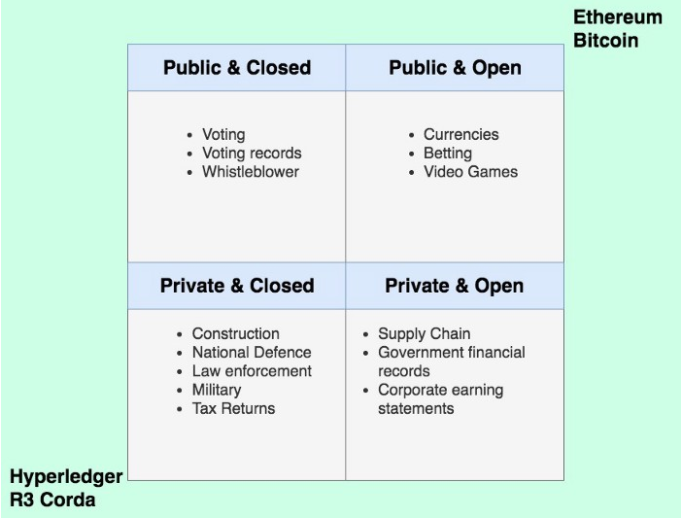
\includegraphics[width=10cm]{imagenes/herramientas/tipos_de_redes}
    \caption{Tipos de redes con sus posibles aplicaciones. Fuente: \cite{public-private-blockchain}}
    \label{fig:tipos-de-redes}
\end{figure}

\vspace{5mm}

\noindent En esta sección vamos a definir los diferentes tipos de redes y sus posibles prácticas.

\subsubsection*{Redes públicas (permissionless).}

Cuando hablamos de redes públicas, nos referimos a redes públicas abiertas. Es un tipo de Blockchain que permite que 
cualquiera pueda unirse a la red, lo que significa que puede leer, escribir o participar en ella. Las Blockchain 
públicas están descentralizadas, nadie tiene control sobre la red, y están seguras de que los datos no pueden ser 
cambiados una vez validados. Este tipo de Blockchain tiende a centrarse más en un escenario B2C o Business to Customer 
\cite{public-private-blockchain}.

\vspace{5mm}

\noindent Las plataformas que podemos encontrar son Bitcoin, Ethereum entre otras criptomonedas. Al no haber permisos,
este tipo de redes se centran en proteger el anonimato de los usuarios y por tanto, no se pueden establecer roles y
controles en qué datos se pueden leer o escribir.

\subsubsection*{Redes privadas (permissioned).}

En contraparte, las redes Blockchain privadas son del tipo cerradas, ya que queremos controlar quien escribe y lee los 
datos de la Blockchain, y por ende tenemos que establecer entidades. Se definen reglas sobre qué datos pueden añadir al 
libro mayor y qué datos pueden consumir del libro mayor. La mayoría de veces, vienen incorporados con herramientas de 
gestión de identidades (OAuth) \cite{public-private-blockchain}. 

\vspace{5mm}

\noindent Las Blockchain privadas también son conocidas como Enterprise Blockchains, ya que son las más utilizadas por 
empresas. Pueden ser Open Source, de consorcio o desarrolladas de forma privada. Las opciones más comunes son 
Hyperledger, R3 Corda y Quorum. Por esta razón, están estructuradas a un modelo B2B o Business to Business. 

\vspace{5mm}

\noindent Las transacciones son procesadas por una cantidad mínina y conocida de nodos de la Blockchain, en comparación 
con las redes públicas, como los 8000 nodos en el caso de Ethereum \cite{ethereum-nodes}. Hay una clara diferencia en 
rendimiento entorno a la latencia y velocidades de transmisión.

\subsubsection*{Beneficios de una red pública.}

\begin{itemize}
\item \textbf{Abierto a lectura y/o escritura}: Cualquiera puede participar enviando transacciones al Blockchain, como 
Ethereum o Bitcoin; las transacciones pueden verse en el explorador del Blockchain.

\item \textbf{El libro mayor es distribuido}: No está centralizado como en un enfoque cliente-servidor, y todos los 
nodos participan en la validación de la transacción.

\item \textbf{Inmutable}.

\item \textbf{Seguro gracias a la minería (regla del 51\%)}: Por ejemplo, con Bitcoin, la obtención de la mayor parte 
de la potencia de la red podría permitir una duplicación masiva de los gastos, y la posibilidad de evitar 
confirmaciones de transacciones, entre otros actos potencialmente malintencionados.
\end{itemize}

\subsubsection*{Beneficios de una red privada.}

\begin{itemize}
\item \textbf{Permisos empresariales}: La empresa controla los recursos y el acceso, por lo tanto, es privada y/o 
autorizada.

\item \textbf{Transacciones más rápidas}: Cuando distribuyes los nodos localmente, y tienes una cantidad mínima de 
nodos, el rendimiento es mejor a la hora de validar las transacciones.

\item \textbf{Mejor escalabilidad}: El hecho de poder añadir nodos y servicios a petición puede ser una gran ventaja 
para la empresa.

\item \textbf{Soporte de cumplimiento}: Como empresa, tiene que satisfacer con requisitos de cumplimiento, y tener el 
control de su infraestructura, esto permite que se cumpla más fácilmente.

\item \textbf{Consenso más eficiente (menos nodos)}: Las Blockchain empresariales o privadas tienen menos nodos y 
suelen tener un algoritmo de consenso diferente, como BFT vs PoW.
\end{itemize}

\subsection{Plataformas Blockchain.}

Conocemos de antemano, que la tecnología Blockchain surgió en 2008 con la plataforma Bitcoin, y ha evolucionado hasta
convertirse en una tecnología dominante, utilizada también a nivel empresarial, y por tanto han surgido nuevas y 
diversas plataformas de Blockchain. En la sección anterior, hemos comentado algunas plataformas, según su tipo de red.
Es el momento de dar paso a definir la lista de las plataformas más conocidas de Blockchain que hay actualmente.

\subsubsection{Plataformas de Blockchain populares.}

\subsubsection*{Hyperledger.}

Hyperledger es conocidad por ser una de las mejores plataformas blockchain de Open-source. Está alojada por la Linux 
Fundation y permite a los usuarios crear y desarrollar frameworks distribuidos de libro de contabilidad a nivel 
empresarial \cite{top-blockchain-platforms}. Se creó en 2015 y hay una amplia gama de frameworks dirigidos a diferentes 
casos de uso \cite{top-blockchain-platforms-app}. Cabe mencionar los siguientes: 
    
\begin{itemize}
    \item \textbf{Hyperledger Fabric}: es un framework de Blockchain para las empresas. Ofrece una amplia gama de 
    características, incluyendo servicios de membresía y consenso. Además, también puede alojar contratos inteligentes 
    llamados \say{chaincode}. IBM y Digital Asses son los primeros en contribuir al proyecto.
    \item \textbf{Hyperledger Sawtooth}: es una plataforma modular, diseñada para desplegar y ejecutar DLT sin una
    autoridad central \cite{top-blockchain-platforms-app2}.
    \item \textbf{Hyperledger Iroha}: es una plataforma de cadena de bloques para la construcción de aplicaciones 
    descentralizadas confiables, seguras y rápidas \cite{top-blockchain-platforms-app2}.
\end{itemize}

\noindent Este tipo de plataforma es permissioned \cite{public-private-blockchain, top-blockchain-platforms-app2}, 
por tanto la entrada a la red de un nuevo participante ha de ser aprobada por el resto de nodos, se crean canales de 
comunicación, donde se implementan la privacidad de transacciones. Se puede catalogar como subredes dentro de la propia 
red.

\subsubsection*{R3 Corda.}

R3 Corda es una plataforma de cadena de bloques de código abierto. Es una tecnología de libro mayor distribuido 
\cite{top-blockchain-platforms-app}.

\vspace{5mm}

\noindent Su enfoque es bastante diferente de la cadena de bloques tradicional, donde una transacción necesita ser 
verificada por muchos nodos. Su enfoque es reducir el número de validaciones y mejorar la eficiencia mientras se 
mantiene intacto todo el conjunto de características de la cadena de bloques \cite{top-blockchain-platforms-app}.

\vspace{5mm}

\noindent Las tres características clave de R3 Corda son el código, diseño y desarrollo abiertos. Cualquiera puede usar 
R3 Corda y utilizar la plataforma de cadena de bloques de código abierto según sus necesidades y requerimientos 
\cite{top-blockchain-platforms-app}. 

\subsubsection*{Ethereum.}

Ethereum es una de las plataformas blockchain más importantes, destacamos de ella ser pionera en los Smart contract así 
como la ejecución simple de los mismos \cite{top-blockchain-platforms-app}. Creada por Vitalk Buterin en 2013, es una 
plataforma de código abierto y pública. Su moneda es el Ether. Sigue un mecanismo de consenso PoW, que es 
comparativamente más lento en velocidad, pero se va a modificar por el algoritmo a prueba de participación o 
Proof-of-Stake\footnote{Proof-of-Stake (PoS) establece que una persona puede minar o validar transacciones dependiendo 
de la cantidad de monedas que tenga. Cuantas más monedas posea un minero, más poder de mineria tendrá.\label{fnlabel}} 
\cite{proof-of-stake}.

\vspace{5mm}

\noindent Ethereum tiene, también, un apartado para empresas conocido como Enterprise Ethereum 
\cite{top-blockchain-platforms}. Ofrece una cadena de bloqueo flexible, segura y escalable dirigida a los negocios. 
Ofrece tres tipos de implementación, incluyendo privada, híbrida y de consorcio. Cualquier empresa puede aprovechar 
las ventajas del Ethereum adaptándolo a sus necesidades. Con las herramientas proporcionadas, puede crear aplicaciones 
descentralizadas (dApp\footnote{Aplicación software que está construida en una red descentralizada \cite{what-is-dapp}.
\label{fnlabel}}). 

\subsubsection*{Quorum.}

Quorum es una plataforma de código abierto diseñada para mejorar la privacidad. Es una innovación basada en Ethereum, 
desarrollada en asociación con J.P. Morgan y EthLab, una startup de Ethereum . Modifica el núcleo de Ethereum y, por lo 
tanto, tiene muchas más características excepcionales añadidas que la tecnología tradicional de cadenas de bloques 
\cite{top-blockchain-platforms-app}. 

\vspace{5mm}

\noindent Esta plataforma permite implementaciones de consensos diferentes según las necesidades. Ofrece privacidad a 
nivel de transacción, junto con transparencia en toda la red, y no soporta la política global de intercambio de datos. 
Actualmente, la platforma de Quórum se está convirtiendo en una parte indispensable de organizaciones como bancos e 
instituciones financieras en las que la privacidad de los datos es crucial \cite{top-blockchain-platforms-app}.

\subsubsection*{Ripple.}

Es una plataforma de cadena de bloques de código abierto que está diseñada para permitir transacciones rápidas y 
baratas. Su criptodivisa es conocida como XRP, pero también permite a la gente crear su propia moneda a través de 
RippleNet. RippleNet permite a los usuarios encontrar nuevos clientes en nuevos mercados, ampliar los servicios y 
ofrecer la mejor experiencia en pagos globales. A diferencia de los métodos de transacción tradicionales, esta 
plataforma tiene por objeto facilitar y agilizar el proceso de transacción, especialmente en el caso de los pagos 
transfronterizos, creando así un mejor ecosistema de crecimiento y desarrollo \cite{top-blockchain-platforms-app}.

\subsubsection{Blockchain como plataformas de servico (BaaS).}

Blockchain-as-a-Service o BaaS, es la creación y gestión por parte de terceros de redes basadas en la nube para 
empresas que se dedican a la construcción de aplicaciones Blockchain. Estos servicios de terceros son un desarrollo 
relativamente nuevo en el creciente campo de la tecnología de las Blockchain, El negocio de la tecnología ha superado 
con creces su uso más conocido en las transacciones en criptografía y se ha ampliado para abordar las transacciones 
seguras de todo tipo \cite{blockchain-as-a-service, top-blockchain-platforms}. Las empresas basadas en la nube que 
implementan la tecnología Blockchain tenemos:

\subsubsection*{IBM.}

IBM es la empresa pionera en aventurarse en la creación de una plataforma Blockchain para operaciones comerciales
transparentes. Posee una división encargada de crear aplicaciones basada en Blockchain \cite{top-blockchain-platforms}.

\vspace{5mm}

\noindent Ofrece una red permissioned, y asegura a las empresas que puedan construir, digirir, operar y crecer usando
la tecnologia de IBM. Soporta Golang y Java.

\subsubsection*{Amazon.}

Amazon también ofrece su solución BaaS con el uso de Amazon Managed Blockchain. Con él, puedes crear y gestionar la 
Blockchain. Funciona con redes de cadenas de bloques populares como Ethereum y Hyperledger Fabric 
\cite{top-blockchain-platforms}.

\vspace{5mm}

\noindent Tiene los siguientes beneficios:

\begin{itemize}
    \item Completamente administrado
    \item Se puede escoger entre Ethereum o Hyperledger Fabric
    \item Seguro y escalable
    \item Confiable
\end{itemize}

\noindent Ofrece una amplia gama de soluciones, incluyendo Amazon QLDB (Quatum Ledger Database), Amazon Managed 
Blockchain, AWS Blockchain Templates, y AWS Blockchain Partners \cite{top-blockchain-platforms}.

\subsubsection{Otras plataformas Blockchain.}

\subsubsection*{OpenChain.}

Es de código abierto y se dirige principalmente a organizaciones que quieren asegurarse de que sus activos digitales
se gestionan y emiten de forma segura, robusta y escalable.

\vspace{5mm}

\noindent Es fácil de usar y administrar, pudiendo establecer reglas para los usuarios finales que participen e 
intercambien el valor definido por esas reglas. Cada transacción está firmada digitalmente para garantizar la 
seguridad. Utiliza el consenso particionado. Cada instancia de Openchain tiene una autoridad para la validez de 
la transacción, en la que la Blockchain utiliza las instancias de Openchain con fines de descentralización. Esto 
significa que la transacción debe ser validada por diferentes instancias de OpenChain \cite{top-blockchain-platforms}.

\vspace{5mm}

\noindent Otras características fundamentales de OpenChain son una mayor eficiencia gracias al uso de una arquitectura 
cliente-servidor y la ausencia de minadores. Por tanton, las transacciones no necesitan ningún tipo de tasas y son 
instantáneas \cite{top-blockchain-platforms-app2}.

\subsubsection*{Stellar.}

Stellar es un libro de contabilidad distribuido basado en cadenas de bloques que se utiliza para facilitar las 
transferencias cruzadas de valor. De manera similar a Ripple, también puede tratar con intercambios entre 
criptodivisas. Es posible construir herramientas bancarias, dispositivos inteligentes y carteras móviles utilizando 
la red Stellar \cite{top-blockchain-platforms-app2}.

\vspace{5mm}

\noindent El Protocolo de Consenso Estelar (SCP) permite llegar a un consenso sin depender de un sistema cerrado de 
registro de las transacciones financieras. Al tener un conjunto de propiedades de seguridad comprobables, el SCP 
optimiza la seguridad deteniendo el progreso de la red hasta que se pueda llegar a un consenso en caso de que los nodos 
o la partición se comporten mal \cite{top-blockchain-platforms-app2}.

\vspace{5mm}

\noindent En comparación con los algoritmos descentralizados de prueba de trabajo y prueba de toma, SCP tiene 
requisitos financieros e informáticos modestos, lo que reduce la barrera de entrada y abre el sistema financiero a 
nuevos participantes \cite{top-blockchain-platforms, top-blockchain-platforms-app2}.

\subsection{Smart Contracts.}

Un contrato inteligente es un acuerdo incrustado en un código informático gestionado por una cadena de bloqueo. El 
código contiene un conjunto de reglas bajo las cuales las partes de ese contrato inteligente acuerdan interactuar entre 
sí. Si se cumplen las reglas predefinidas, el acuerdo se cumple automáticamente. Los contratos inteligentes 
proporcionan mecanismos para gestionar eficazmente los activos simbólicos y los derechos de acceso entre dos o más 
partes \cite{what-is-smart-contract}. 

\vspace{5mm}

\noindent Pueden formalizar las relaciones entre personas e instituciones y los bienes que poseen a través de Internet, 
totalmente P2P, sin necesidad de intermediarios de confianza. La tecnologías de Blockchain son impulsores del concepto 
para la implementación de contratos inteligentes.

\vspace{5mm}

\noindent Los contratos inteligentes, proporcionan una forma pública y verificable de integrar las reglas de gobierno y 
la lógica empresarial en unas pocas líneas de código, que pueden ser auditadas y aplicadas por el consenso mayoritario 
de una red P2P \cite{what-is-smart-contract}.

\vspace{5mm}

\begin{figure}[ht!]
    \centering
    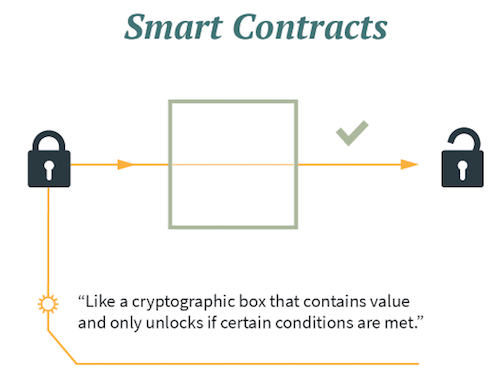
\includegraphics[width=8cm]{imagenes/herramientas/smart-contracts}
    \caption{Ejemplo de Smart-Contract con contenido criptográfico. Fuente: \cite{what-is-smart-contract}}
\end{figure}

\vspace{5mm}

\noindent Un contrato inteligente puede ser invocado desde entidades dentro (otros contratos inteligentes) y fuera 
(fuentes de datos externas) de la Blockchain. Los contratos inteligentes podrían proporcionar una seguridad en las 
transacciones superior a la del derecho contractual tradicional, con lo que se reducirían los costos de coordinación 
de la auditoría y el cumplimiento de esos acuerdos \cite{what-is-smart-contract}. 

\subsubsection*{Casos de uso.}

Los casos de uso de contratos inteligentes van de simples a complejos. Pueden utilizarse para transacciones económicas 
sencillas como el envío de dinero de A a B. También pueden utilizarse para registrar cualquier tipo de propiedad y de 
derechos de propiedad, como los registros de tierras y la propiedad intelectual, o para gestionar el control de acceso 
inteligente para la economía de reparto. Se pueden encontrar casos de uso en la banca, los seguros, la energía, el 
gobierno electrónico, las telecomunicaciones, la industria musical, el arte, la movilidad, la educación y muchos más 
\cite{what-is-smart-contract}.

\subsection{Herramientas utilizadas para desarrollo del proyecto.}

En esta sección vamos a comentar las herramientas utilizadas en el proyecto y el motivo de por qué he utilizado dichas
herramientas para cada apartado de la prueba de concepto. Como ya conocemos en la sección \ref{motivacion}, comenté 
sobre los dispositovs que voy a utilizar, que son Rasberry Pi para simular la red Blockchain y los dispositivos IoT que 
se encargarán de interactuar con la red. Y para la elaboración de la aplicación he decido implementar una aplicación 
web que constará de dos partes principalmente. Una API\footnote{Una interfaz de programación de aplicaciones es una 
interfaz informática que define las interacciones entre múltiples intermediarios de software. Define los tipos de 
llamadas o solicitudes que pueden hacerse, cómo hacerlas, los formatos de datos que deben utilizarse, las convenciones 
a seguir, etc \cite{api}.\label{fnlabel}} para hacer consultas directamente a la red Blockchain y un Front end para la 
visualización de los datos obtenidos desde la API hasta el cliente. 

\vspace{5mm}

\noindent Las aplicaciones basadas en la web son un tipo de software que permite a los usuario interactuar con un 
servidor remoto a través de una interfaz de navegador web \cite{web-based-app}. Con el paso de los años, ha tomado 
mucha relevancia y popularidad, sustituyendo a las aplicaciones de escritorio. Tienen varias ventajas sobre las 
aplicaciones de escritorio tradicionales, una de ellas es la portabilidad. Con las aplicaciones basadas en la web, 
los usuarios no tienen que instalar software adicional y los desarrolladores no tienen que escribir múltiples versiones 
de la misma aplicación para diferentes sistemas operativos o plataformas \cite{web-based-app}, tan sólo se deben de 
preocupar de las compatibilidades de los diferentes navegadores que hay actualmente (Chrome, Mozilla Firefox, Safari, 
Opera, etc).

\vspace{5mm}

\noindent Otras ventajas que ofrece las aplicaciones basadas en web son: 

\begin{itemize}
    \item Son \textbf{multiplataforma} y \textbf{acceso universal}, para todos los sistemas operativos y móbiles
    \item \textbf{Accesibles} en cualquier momento, siempre y cuando se tenga acceso a internet. Aunque como veremos 
    más adelante, podremos interactuar con la aplicación de manera \textbf{offline}, gracias a PWA (Progressive Web 
    Application).
    \item \textbf{Ahorro en tiempo y dinero}, al no tener que elaborar la aplicación para múltiples plataformas y 
    lenguajes.
    \item Son \textbf{altamente escalables}. Es fácil aumentar rápidamente la cantidad de usuarios activos, ya que 
    no tiene que ser instalado y configurado. También, gracias a balanceadores de carga para administar clústeres,
    permite alta disponibilidad y sin tiempos de inactividad \cite{swap}. 
    \item Son excelentes para almacenar datos. Los datos son almacenados en la nube, y es el servidor el que se 
    encarga de gestionar la información y distribuirla a los usuarios.
    \item Son \textbf{seguras}.
    \item El despliegue es fácil, rápido y fáciles de actualizar y mantener.
\end{itemize}

\noindent Estas ventajas de las aplicaciones web para empresas han permitido que el software basado en la web gane 
popularidad tanto en las corporaciones multinacionales como en las pequeñas empresas. Por tanto, son buenos los 
motivos para utilizar las aplicaciones web, para la implementación del proyecto.

\vspace{5mm}

\noindent Anteriormente, hemos mencionado el concepto de PWA. Se trata de un tipo de aplicación software que se entrega
a través de la web, y diversas compañias como Google, Microsoft, Mozilla y Apple, están implementando soporte para ello. 
Estás aplicaciones son aplicaciones web, pero se comportan más como aplicaciones nativas. Al instalar una aplicación 
web progresiva (ver fig.\ref{fig:instalacion-pwa}), se podrá tener un acceso directo desde la pantalla de inicio, en la 
barra de tareas o en el escritorio. La aplicación se cargará rápidamente e incluirá soporte fuera de línea, 
notificaciones y soporte de sincronización en segundo plano \cite{progressive-web-apps}. 

\vspace{5mm}

\begin{figure}[ht!]
    \centering
    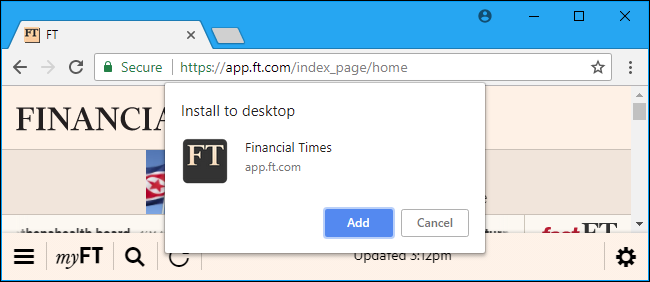
\includegraphics[width=8cm]{imagenes/herramientas/pwa-instalacion}
    \caption{Ejemplo de instalación de una PWA en el escritorio. Fuente: \cite{progressive-web-apps}}
    \label{fig:instalacion-pwa}
\end{figure}

\vspace{5mm}

\noindent Este último concepto, ha permitido que aparte de elaborar una aplicación web, poder tener una aplicación 
tanto para el escritorio como para el móvil\footnote{La aplicación ha de ser responsive, para que se pueda adaptar a 
cualquier tamaño de pantalla.\label{fnlabel}} y poder utilizarla sin necesidad de un navegador, ni instalaciones y con 
todas las ventajas que ofrece las aplicaciones web progresivas. 

\subsubsection{Implementación de la red Blockchain.}

Teniendo en cuenta los objetivos del proyecto para la gestión y administración de dispositivos IoT de una red
domótica, era necesario utilizar una tecnología Blockchain privada, para identificar qué dispositivos están
escribiendo o leyendo datos y llevar un control de todos ellos. Por tanto, la tecnología que hemos escogido 
para el proyecto es Hyperledger Fabric, ya que se basa en una red autorizada, y por tanto los participantes
han de estar autenticados. También posibilita la creación de contratos inteligentes (chaincode), para poder 
implementar la lógica de la red. También consta de la creación de canales privados entre los nodos seleccionados 
para ejecutar la lógica del chaincode sobre el canal, protegiendo los datos \cite{why-hyperledger-fabric}.

\vspace{5mm}

\noindent Hyperledger Fabric ofrece un número de SDKs\footnote{SDK significa software development kit o devkit. Es un
conjunto de herramientas de software y programas utilizados por los desarrolladores para crear aplicaciones para 
plataformas específicas \cite{what-is-sdk}.\label{fnlabel}} para apoyar el desarrollo de contratos 
inteligentes en varios lenguajes de programación. Hay tres disponibles: Go, Node.js y Java. En cuanto al desarrollo 
de aplicaciones soporta los lenguajes de Node.js y Java pero actualmente, aunque en desarrollo, tienen Python y Go 
\cite{hyperledger-fabric-docs, hyperledger-fabric-nodejs-sdk}.

\vspace{5mm}

\noindent En esta ocasión, hemos escogido, Go para la creación de los chaincode y para la parte de la elaboración
de la API, nos hemos decantado por Node.js, que más adelante comentaremos en la siguiente sección. Los chaincode 
se ejecutan en un contenedor Docker seguro y aislado del proceso de aprobación de los peers. Inicializa y gestiona 
el estado del libro mayor a través de las transacciones presentadas por las solicitudes. Se puede invocar un 
chaincode dentro de un mismo canal para actualizar y consultar el libro mayor, con los permisos correspondientes.

\vspace{5mm}

\noindent Hyperledger Fabric también necesita que tengamos instalado Docker y Docker Compose, para la gestión de los 
diferentes componentes que podemos crear en nuestra red privada. Al ser un arquitectura modular, dichos componentes 
toman diferentes roles dentro de la red privada \cite{hyperledger-fabric-docs}. Vamos a comentar uno por uno de los 
elementos y su labor dentro de una red:

\begin{itemize}
    \item \textbf{Peer}: Mantiene el libro mayor y ejecuta contenedores de chaincode para realizar operaciones de 
    lectura/escritura.
    \item \textbf{Ordering Service (Servicio de pedidos)}: El servicio de pedidos se encarga de mandar los bloques de 
    las transacciones para todos los canales de la red y que sean consumidos por los peers. Tambíen genera el bloque 
    génesis. Esto lo rige el componente \textbf{Orderer}.
    \item \textbf{CA}: La autoridad certificadora de Hyperledger Fabric es el componente predeterminado de la 
    Autoridad de Certificación, que emite certificados basados en la PKI a las organizaciones miembros de la red y a 
    sus usuarios. La CA emite un certificado raíz (rootCert) a cada miembro y un certificado de inscripción (ECert) a 
    cada usuario autorizado.
    \item \textbf{CLI (Command Line Interface)}: Hyperledger Fabric posee un CLI para realizar operaciones establecidas 
    en los chaincode dentro de nuestra red. Requiere que esté vinculado a un peer de la red.
\end{itemize}

\noindent A la hora de guardar las transacciones, Hyperledger Fabric ofrece dos tipo de bases datos, LevelDB y CouchDB. 
LevelDB es la base de datos de estado predeterminada e incrustada en el nodo peer y almacena los datos del chaincode 
como pares clave-valor simples y sólo admite consultas clave, rango clave y clave compuesta. En cambio, CouchDB es 
opcional y soporta consultas ricas ya que los datos de los chaincode están en formato JSON. Los datos se encuentran 
indexados, lo que hace que las consultas sean flexibles y eficientes \cite{using-couchdb}.

\vspace{5mm}

\noindent Antes de la creación de la red, es necesario establecer qué base de datos se quiere utilizar, en mi caso, me 
he decantado por utilizar CouchDB por todos los beneficios mencionados anteriormente.

\vspace{5mm}

\noindent Con Docker y Docker Compose, nos permite crear contenedores ligeros para ejecutar cada componente de la red, 
con la ventaja de ser cada uno portable y seguro por la capacidades de aislamiento que tienen. Con Docker Compose 
podemos definir y ejecutar aplicaciones de varios contenedores Docker. Y mediante comandos, podemos crear e iniciar 
todos los servicios que estén configurados.

\vspace{5mm}

\noindent Al utilizar varias Raspberries como nodos principales de la red Blockchain, como un clúster, voy a utilizar 
Docker Swarm para la orquestación de multiples contenedores dentro de múltiples máquinas anfitrionas. Dentro de un 
clúster hay varios nodos trabajadores y un nodo administrador que se encarga de manejar los recursos de los nodos 
trabajadores de manera eficiente y de asegurar que el grupo funcione con eficacia. También, hace que la aplicación 
tenga un alto nivel de disponibilidad \cite{what-is-docker-swarm}.

\subsubsection{Herramientas para el Back end.}

\subsubsection*{GraphQL.}

En esta sección hablaremos sobre la creación de la API con Node.js y utilizando el estandar de GraphQL. GraphQL es un 
lenguaje de código abierto de consulta y manipulación de datos para APIs. Fue desarrollado por Facebook en 2012 y 
publicado en 2015 \cite{graphql}. Hoy en día REST se ha convertido en una estandar para el diseño de web APIs. Sin 
embargo, es inflexible a la hora de obtener los datos según lo que solicita el cliente. Con REST es necesario realizar 
varias llamadas a diferentes endpoints con estructura de datos fijas (ver fig.\ref{fig:consulta-rest}), y por tanto se 
produce insuficiencia o exceso de los datos que realmente se requieren \cite{graphql-vs-rest}. 

\begin{figure}[ht!]
    \centering
    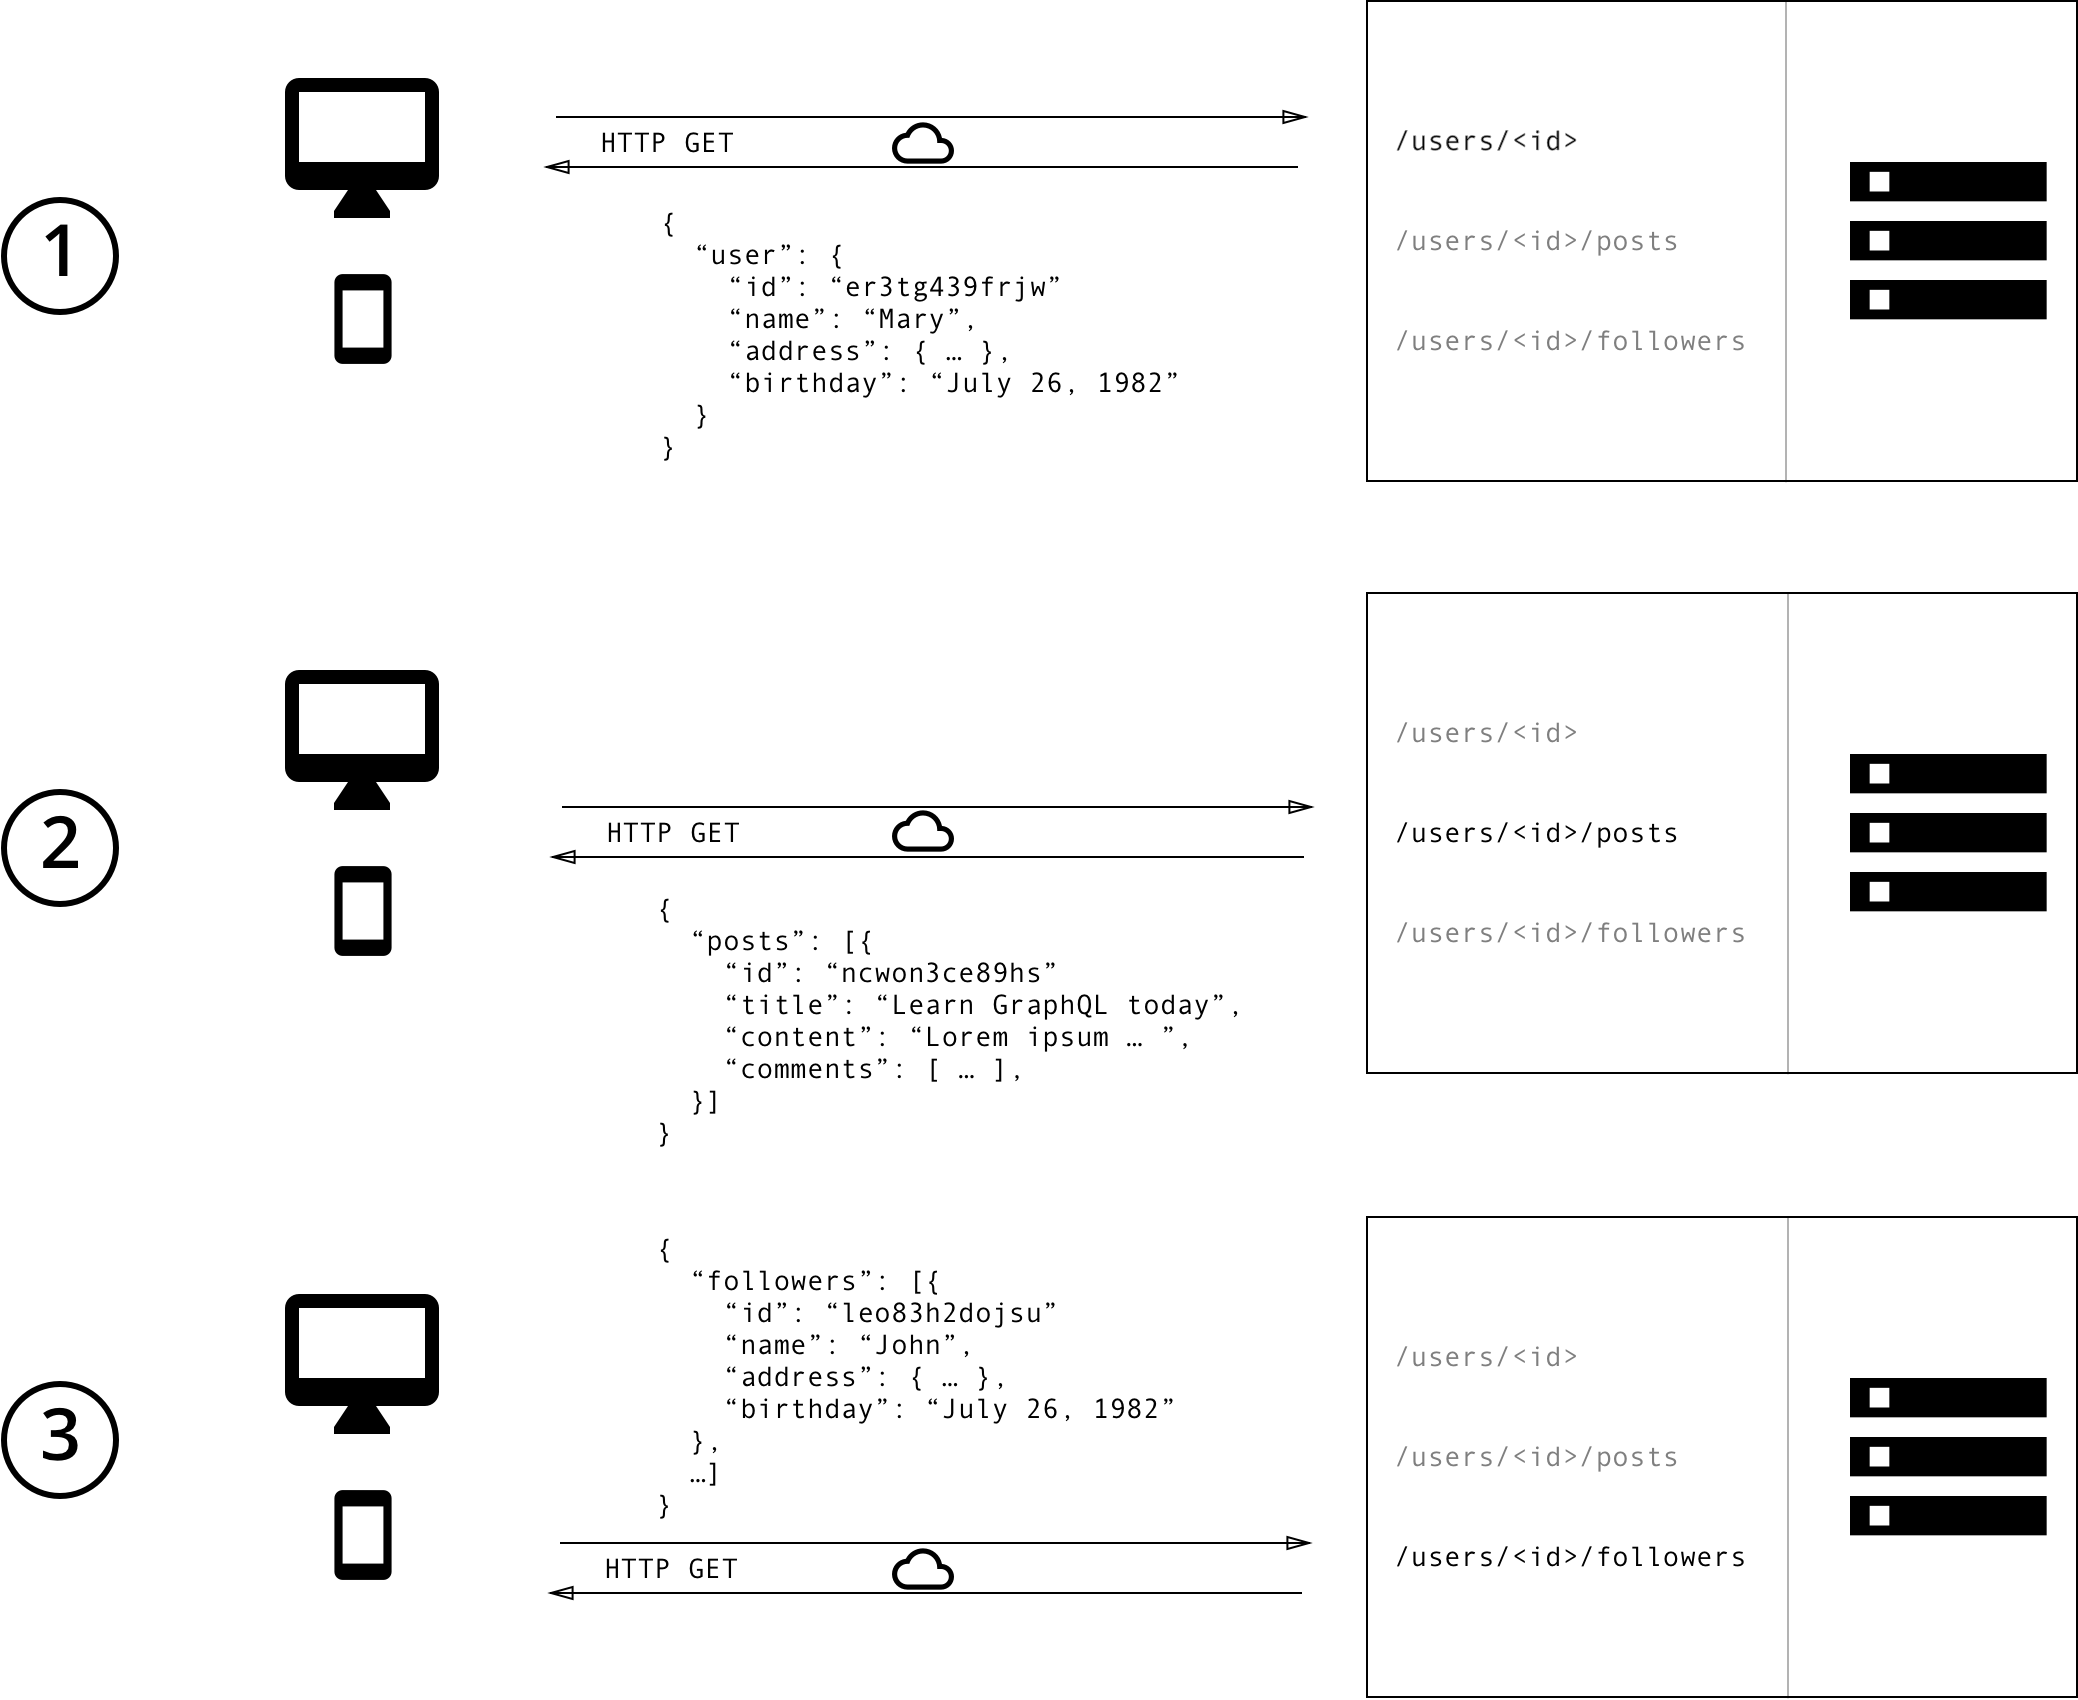
\includegraphics[width=12cm]{imagenes/herramientas/rest-query}
    \caption{Tres llamadas a endpoints de un REST API para solicitar los datos necesarios. Fuente: 
    \cite{graphql-vs-rest}}
    \label{fig:consulta-rest}
\end{figure}

\vspace{5mm}

\noindent Gracias a GraphQL, basta con mandar solo una consulta con los datos que se quiera en concreto, y el 
servidor responde con un objeto JSON con los requerimientos rellenos (ver fig.\ref{fig:consulta-graphql}) 
\cite{graphql-vs-rest}.

\vspace{5mm}

\begin{figure}[ht!]
    \centering
    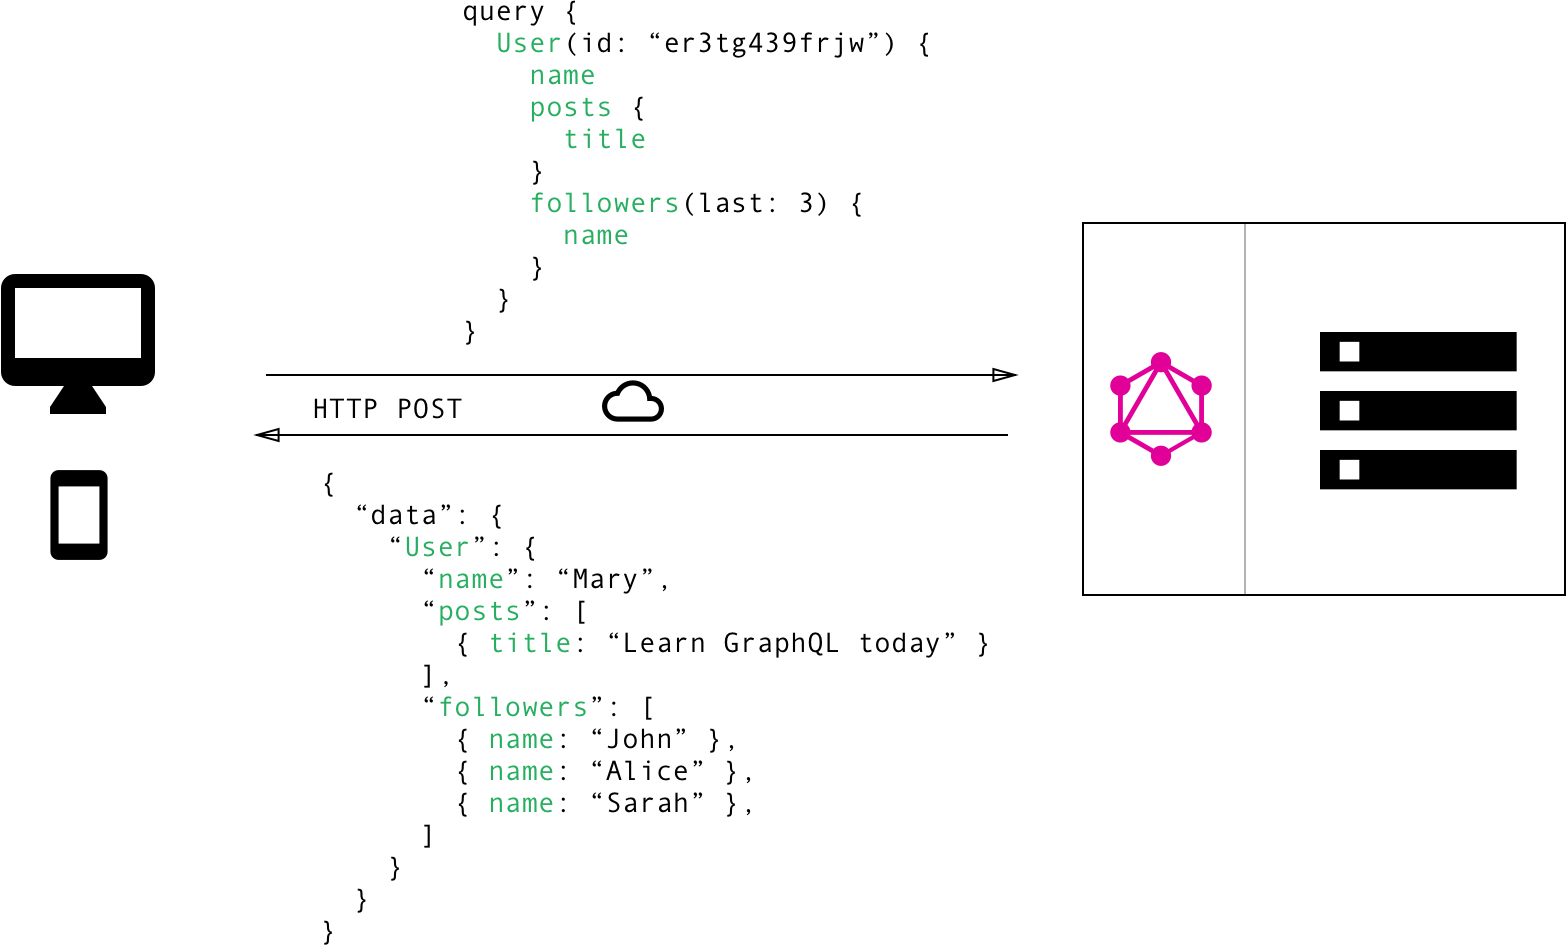
\includegraphics[width=12cm]{imagenes/herramientas/graphql-query}
    \caption{Una única llamada para solicitar los datos necesarios. Fuente: \cite{graphql-vs-rest}}
    \label{fig:consulta-graphql}
\end{figure}

\vspace{5mm}

\noindent En GraphQL es necesario definir esquemas para indicar las capacidades de una API. Una vez definido el esquema, 
tanto el Front como el Back son conscientes de la estructura definitiva de los datos.

\subsubsection*{Node.js}

Node.js es un entorno de ejecución que permite ejecutar código JavaScript fuera del navegador, utilizando Chrome V8 
como motor de JavaScript. Este entorno permite escribir comandos de línea en una terminal y \say{scripting} en el lado 
del servidor \cite{what-is-nodejs}.

\vspace{5mm}

\noindent Usa un gestor de paquetes JavaScript por defecto, llamado NPM (Node Package Manager). Fue fundada en 2014 y
adquirida por Github en 2020. Es un proyecto de código abierto para ayudar a los desarrolladores de JavaScript a
compartir fácilmente módulos de código empaquetado. Mantiene una colección pública de paquetes de código abierto
para Node.js, aplicaciones web de front-end, aplicaciones para móvil, robots, enrutadores, etc. El cliente de línea 
de comandos permite a los desarrolladores instalar y publicar esos paquetes.

\vspace{5mm}

\noindent La razón por el cual he escogido Node.js es por utilizar el SDK que ofrece Hyperledger Fabric para la 
creación de aplicaciones sobre redes Blockchain, por la buena comunidad que tiene el lenguaje y la cantidad de 
paquetes que ofrece, lo que facilita el desarrollo de la aplicación web.

\vspace{5mm}

\noindent Entre los paquetes los paquetes que he instalado en el lado del servidor caben destacar:

\begin{itemize}
    \item \textbf{fabric-network}: envio de transacciones y consultas de contratos inteligentes.
    \item \textbf{fabric-ca-client}: contiene los servicios para la administración de usuarios, añadir, revocar por ID
    o por certificado, y se puede personalizar la persistencia.
    \item \textbf{graphql}: necesario para la implementación de la API de lenguaje de consulta de JavaScript. 
    \item \textbf{Apollo Server}: creación de servidor GraphQL y es compatible con Apollo Client. Permite definir 
    esquemas con literales de GraphQL \cite{introduction-apollo-server}. Es un complemento para el middleware Node.js 
    como Express. Tiene una buena documentación.
    \item \textbf{Express}: es framework web ligero para ayudar a organizar una aplicación web en una arquitectura MVC 
    en el lado del servidor \cite{what-is-express.js}.
\end{itemize}

\subsubsection*{SDK Node.js de Hyperledger Fabric.}

\noindent El SDK que ofrece Hyperledger Fabric de Node.js, permite interactuar con la red Blockchain de Hyperledger
utilizando los certificados TLS para asegurar el envio de solicitudes. La seguridad de la red se hace con firmas
digitales. Un usuario se considera válido, si está firmado por un CA (autoridad de certificación) de confianza.

\vspace{5mm}

\noindent Con SDK de Node.js se pueden ejecutar las siguientes acciones:

\begin{itemize}
    \item Crear canales.
    \item Pedir a los nodos iguales que se unan al canal.
    \item Instalar chaincodes en pares.
    \item Instanciar códigos de cadena en un canal.
    \item Invocar transacciones llamando al chaincode.
    \item Consultar el libro mayor para transacciones o bloques.
\end{itemize}

\subsubsection{Herramientas para el Front end.}

Tras hablar sobre las herramientas y frameworks utilizados en el lado del servidor, en esta sección vamos a hablar 
sobre las herramientas utilizadas en el lado del cliente.

\subsubsection*{Gatsby.}

Gatsby es un generador de sitios estáticos basado en React, alimentado por GraphQL. Utiliza las mejores partes de 
React, webpack, react-router, GraphQL, y otras herramientas de cliente \cite{gatsby, what-is-gastby.js}.

\vspace{5mm}

\noindent Utiliza una poderosa preconfiguración para construir un sitio web que utiliza sólo archivos estáticos para 
cargas de página increíblemente rápidas, trabajadores de servicio, división de código, renderizado del lado del 
servidor, carga inteligente de imágenes, optimización de activos y pre-recolocación de datos 
\cite{what-is-gastby.js, why-gatsby}.

\vspace{5mm}

\noindent Gatsby está muy bien integrado con GraphQL para construir su capa de datos. Permite recopilar datos desde 
donde sea que estén: Markdown, JSON, CMS, APIs de terceros, etc. Y en el momento de la construcción, crea un servidor 
interno de GraphQL de todos estos datos. Todos los componentes de React se construyen mediante consultas a través de 
GraphQL.

\vspace{5mm}

\noindent Cuenta con una gran documentación y riqueza de plugins que puedes añadir a tu aplicación web. Está dedicado 
al rendimiento y a la accesibilidad, permitiendo crear PWA de manera sencilla y fácil \cite{why-gatsby}.

\vspace{5mm}

\noindent React es una biblioteca creada por Facebook, basada en JavaScript, que permite construir interfaces de 
usuario mediante componentes y dispone de una gran cantidad de documentación con una buena comunidad por detrás 
\cite{react}.

\vspace{5mm}

\noindent Existen diversas tecnologías similares a React, como Angular o Vue. Angular es un framework más maduro, 
creada por Google que tiene un buen respaldo en términos de contribuyentes, sin embargo, su curva de aprendizaje es 
empinada y más compleja que React. Vue no tiene respaldo de ninguna compañia importante, se fundamenta por 
contribuyentes al proyecto. Posee menos documentación y es menos conocido \cite{angular-react-vue}. 

\vspace{5mm}

\noindent También se ha utilizado Apollo Client, que es una biblioteca completa de gestión de estado para JavaScript 
que permite gestionar datos locales y remotos con GraphQL. Sirve para obtener, almacenar y modificar datos de 
aplicaciones, mientras se actualiza la interfaz de usuario. El núcleo de la biblioteca de Apollo Cliente, proporciona 
una integración con React y Apollo Server \cite{introduction-apollo-client}.

\subsubsection*{Bootstrap.}

Bootstrap es un framework código abierto y gratuito de CSS dirigido al desarrollo de la web móvil. Contiene 
plantillas de diseño basadas en CSS y (opcionalmente) en JavaScript para la tipografía, los formularios, los botones, 
la navegación y otros componentes de la interfaz \cite{bootstrap}.

\vspace{5mm}

\noindent Se ha utilizado la biblioteca Reactstrap que contiene componentes de React Bootstrap 4 que favorecen la 
composición y el control \cite{reactstrap}.

\vspace{5mm}

\noindent Para este proyecto, se ha elegido Bootstrap porque tiene un patrón más dirigido al diseño responsive, 
adaptado a dispositivos móviles, que frameworks de su competencia como Materialize.

\subsection{Conclusión.}

Los temas que hemos tratado en este capítulo son: los tipos de redes Blockchain dependiendo del uso que se quiere 
llevar a cabo, también se ha indagado en las plataformas más conocidas que se utilizan hoy en día basadas en la 
tecnología Blockchain, tanto para uso personal como empresarial. Se ha tratado sobre el concepto de Smart Contract, 
como sistema sustituto a los métodos tradicionales. Finalmente, hemos comentado sobre las herramientas que se han 
escogido para la elaboración de la red Blockchain y para la aplicación web.

\newpage